\documentclass{beamer}

\mode<presentation>{
\usetheme{PaloAlto}
%\usetheme{Berlin}
\usecolortheme{default}
\usefonttheme{professionalfonts}
}

\usepackage[utf8]{inputenc}
\usepackage{babel}
\usepackage{graphicx}
\usepackage{booktabs}
\usepackage{svg}
\usepackage{url}
\usepackage{appendixnumberbeamer}
\usepackage{hyperref}

\usepackage{physics}
\graphicspath{{figs}}
%\usepackage{relsize}
\usepackage{amsmath}
\usepackage{commath}
\usepackage{subcaption}
\usepackage{xfrac}
\usepackage{xcolor}

\title{The Hubbard Model in Low Dimensions}
\author{Christoph Gäntgen and Ulli Pohl}
\institute[]{Physikalisches Institut\\
	Rheinische Friedrich-Wilhelms-Universität Bonn}
\date{March 31st 2020}


\makeatletter
\setbeamertemplate{sidebar \beamer@sidebarside}%{sidebar theme}
{
	\beamer@tempdim=\beamer@sidebarwidth%
	\advance\beamer@tempdim by -6pt%
	\insertverticalnavigation{\beamer@sidebarwidth}%
	\vfill
	\ifx\beamer@sidebarside\beamer@lefttext%
	\else%
	\usebeamercolor{normal text}%
	\llap{\usebeamertemplate***{navigation symbols}\hskip0.1cm}%
	\vskip2pt%
	\fi%
}%
\makeatother
%\setbeamersize{sidebar width left = 3.6em}

\begin{document}

\begin{frame}
\titlepage
\end{frame}

\begin{frame}
\frametitle{Inhalt}
\tableofcontents
\end{frame}

\section{Motivation}
\begin{frame}
\frametitle{Motivation}
\begin{itemize}
	\item Simplified model - still exhibits interesting physics 
	\item Examples: metal-insulator transition, antiferromagnetism and superconductivity
	\item Exact diagonalization is too time-/storageexpensive $\rightarrow$ Monte Carlo Integration
\end{itemize}
\end{frame}

\section{Theoretical background}
\subsection{Hubbard model}
\begin{frame}
\frametitle{Hubbard model - A simplified model}
\begin{figure}[h]
	\centering
	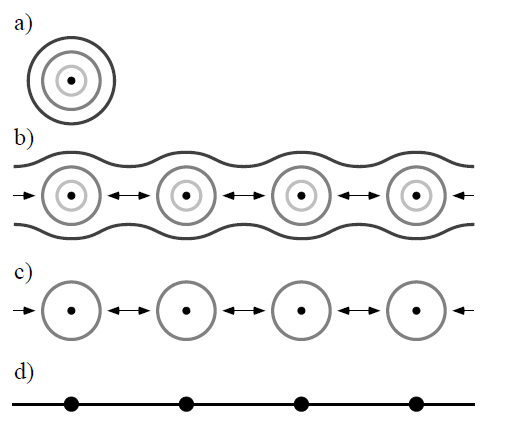
\includegraphics[width=0.6\linewidth]{pic0}
	\caption{From valence electrons and bound electrons to the Hubbard simplification}
	\label{fig:pic0}
\end{figure}
\end{frame}

\begin{frame}
	\frametitle{Hubbard model - 2}
	\begin{figure}[h]
		\centering
		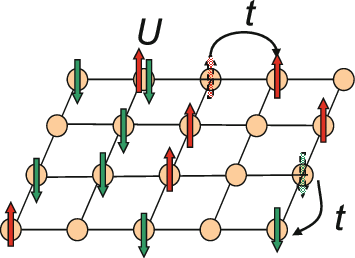
\includegraphics[width=0.4\linewidth]{pic2}
		\caption{Illustration of the model on a 2D lattice}
		\label{fig:pic2}
	\end{figure}
	\begin{equation*}\label{Hubbard_standard}
	H = -t\sum_{\langle ij\rangle,\sigma}\left( c_{i\sigma}^\dag c_{j\sigma} + c_{j\sigma}^\dag c_{i\sigma}\right) + U \sum_{i}n_{i\uparrow}n_{i\downarrow}
	\end{equation*}
\end{frame}

\begin{frame}
\frametitle{Hubbard model - Fock space}
\begin{itemize}
\item Fock space containing all many body states of the Hamiltonian
\item Example 1 site lattice: \[ \ket{0},\; \ket{\uparrow},\; \ket{\downarrow}\; \text{oder} \; \ket{\uparrow\downarrow}\]
\item For $L$ lattice sites $ 4^L $ possible states, but
\end{itemize}
\[ H=\left( \begin{array}{ccc}
H_{N=0}  & 0 & 0\\
0 & H_{N=1} & 0\\
0 & 0 & H_{N=2}\\
\end{array}\right)  \]
$ \Rightarrow $ Basis splits up

\end{frame}

%\begin{frame}
%\frametitle{Impuls-Basis}
%Diagonalisierter hopping-Term:
%\[ H_0 = \sum_{\boldsymbol{k} \sigma} \epsilon_{\boldsymbol{k}} c_{\boldsymbol{k}\sigma}^\dag c_{\boldsymbol{k}\sigma} \]
%Fourier-transformierte Operatoren:
%\[ c_{\boldsymbol{k}\sigma} = \frac{1}{\sqrt{N}}\sum_{j} e^{i\boldsymbol{k}\boldsymbol{R}_j} c_{j\sigma}, \qquad c_{\boldsymbol{k}\sigma}^\dagger = \frac{1}{\sqrt{N}}\sum_{j} e^{-i\boldsymbol{k}\boldsymbol{R}_j} c_{j\sigma}^\dagger \]
%Impulszustand:
%\[ \ket{a(k)} = \frac{1}{\sqrt{N_a}}\sum_{r=0}^{N-1}e^{-ikr}T^r\ket{a} \]
%\end{frame}

\subsection{Correlation functions}
\begin{frame}
\frametitle{Correlation functions}
\begin{itemize}
	\item Partition function 
	\begin{equation*}
	Z := \text{Tr}(\text{e}^{-\beta H}) = \sum_{n}^{}\text{e}^{-\beta E_n} \label{partition}
	\end{equation*}
\item Energy expectation value
\begin{equation}
\langle{E}\rangle = \frac{1}{Z}\text{Tr} (H\text{e}^{-\beta H}) =\frac{1}{Z} \sum_{n}^{} E_n\text{e}^{-\beta E_n} \label{energy}
\end{equation}	
\item Correlator
\begin{equation}
\braket{C_{\alpha\beta}(\tau)}= \frac{1}{Z}\sum_{i}^{}\braket{i|a_{\alpha}(\tau)a^{\dagger}_{\beta}(0)|i}	\label{correlator}
\end{equation}
\end{itemize}
%Die Selbstkonsistenz-Bedingung muss erfüllt sein
\end{frame}
\subsection[Analytic solutions]{Analytic solution for small lattices}
\begin{frame}
\frametitle{Analytic solution of the model for small lattices}
\begin{itemize}
\item For 1 (2) lattice sites only 4(16) states in Fock space
\item can find expressions for correlaors analytically
\end{itemize}
\end{frame}



\begin{frame}
\frametitle{Solving the 1 site model}

\begin{figure}[h]
	\centering
	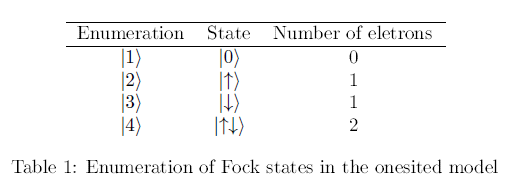
\includegraphics[width=0.7\linewidth]{states}
	\label{fig:states1}
\end{figure}
\begin{equation*}
\langle i|H|j\rangle=
\begin{pmatrix}
0 & 0 & 0&0\\
0 & -\frac{U}{2} & 0&0\\
0 & 0 & -\frac{U}{2}&0\\
0 & 0 & 0&0
\end{pmatrix}
\end{equation*}
\begin{equation}
Z_{1}= 2 (1+\text{e}^{\beta U/2})
\label{partition1}
\end{equation}
\end{frame}


\section{Methods}
\begin{frame}
	\frametitle{Methods}
	\begin{itemize}
		\item Hubbard-Stratonovich transformation
		\item Importance sampling
	\end{itemize}
\end{frame}

\subsection{Hubbard-Stratonovich transformation}
\begin{frame}
\frametitle{Hubbard-Stratonovich transformation}
\begin{itemize}

\item Calculating expectation values
\begin{align*}\label{Pathintegral}
\langle O(t)\rangle &= \frac{1}{Z} \operatorname{Tr}\left[O(t) e^{-\beta H}\right]\\ &=
\frac{1}{Z} \int\left[\prod_{i} d \psi_{i}^{\dagger} d \psi_{i}\right] e^{-\Sigma_{j}\left(\psi_{j}^{\dagger} \psi_{j}\right)}\bra{-\psi}O(t) e^{-\beta H}\ket{\psi}
\end{align*}
\end{itemize}
\end{frame}

\begin{frame}
	\frametitle{Hubbard-Stratonovich transformation - 2}
	\begin{itemize}
		
		\item Trick to reduce the number of fermion fields
		\begin{equation*}\label{linearize}
		e^{\frac{1}{2} U n^{2}}=\frac{1}{\sqrt{2 \pi U}} \int_{-\infty}^{\infty} d \phi\: e^{-\frac{1}{2 U} \phi^{2} \pm \phi n}
		\end{equation*}
		\item Correlator:
		\begin{equation*}\label{C}
		C_{\alpha\beta}(\tau) =\lim _{N_{t} \rightarrow \infty} \int_{-\infty}^{\infty} \mathcal{D}[\phi]\:e^{-\frac{1}{2 \tilde{U}} \phi^2}M^{-1}_{\alpha\tau,\beta 0}[\phi]\det(M[\phi]M[-\phi])
		\end{equation*}
	\end{itemize}
\end{frame}
\subsection{Importance sampling}
\begin{frame}
\frametitle{Importance sampling}
	\begin{itemize}
		\item  $\sqrt{2\pi\tilde{U}}^{-1}$ included in $\mathcal{D}[\phi]$ $\Rightarrow$ sample from $\mathcal{N}_{0, \sqrt{\tilde{U}}}$
		\item Then calculate matrix part and average
	
\end{itemize}
\end{frame}

\begin{frame}
	\frametitle{Importance sampling - 2}
	\begin{figure}[h]
		\centering
		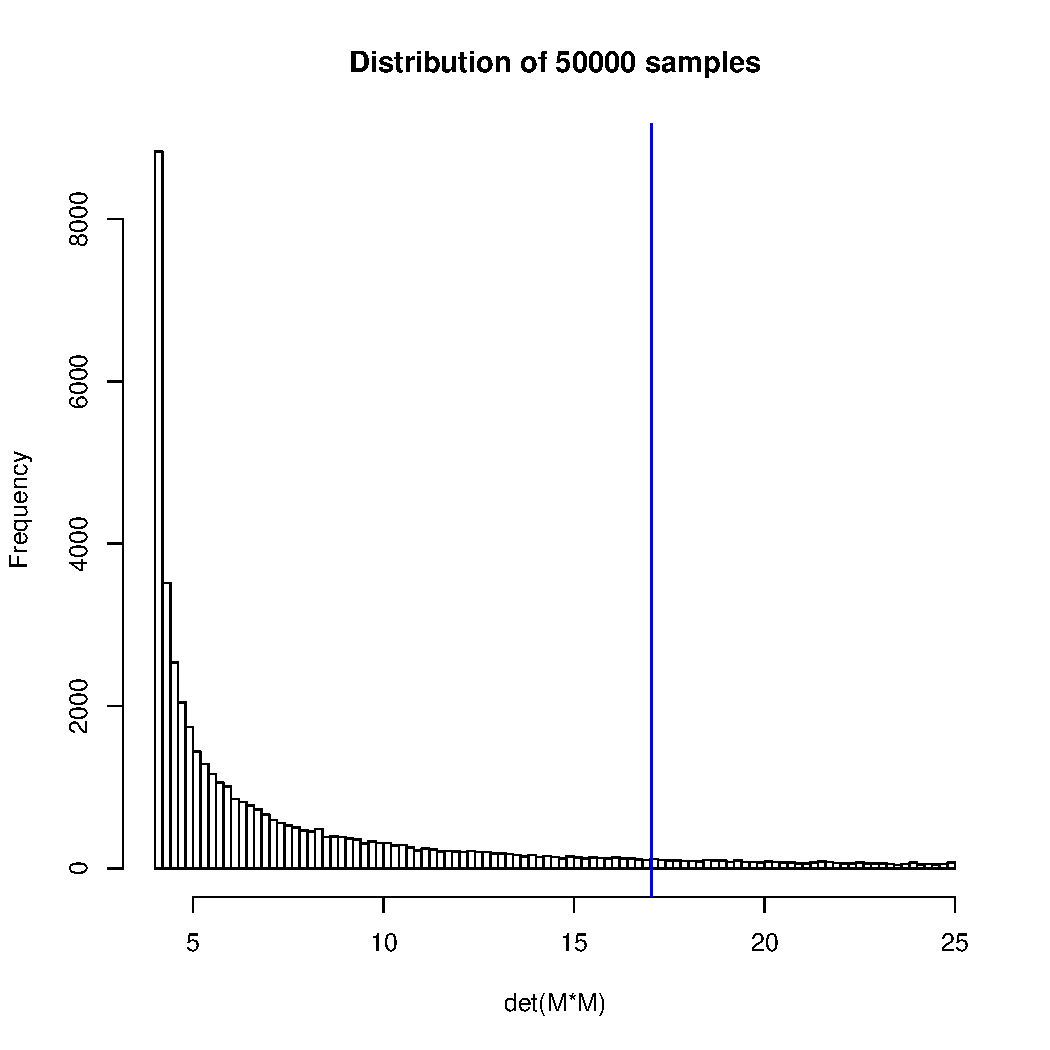
\includegraphics[width=0.9\linewidth]{figs/distribution}
	\end{figure}
\end{frame}
\section{Results}

\begin{frame}
	\frametitle{Results - Partition function}
		\begin{figure}
			\centering
			\begin{minipage}{.5\textwidth}
				\centering
				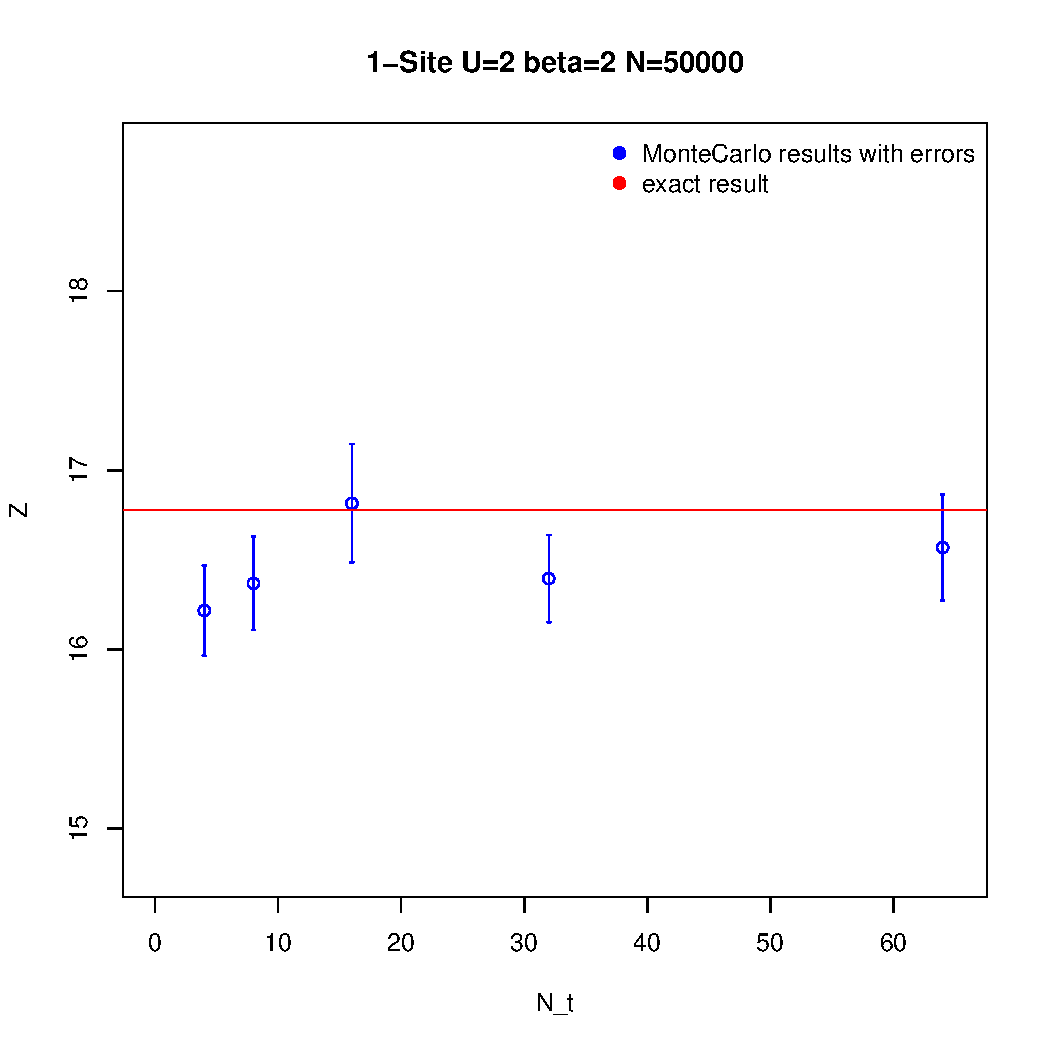
\includegraphics[width=1\linewidth]{figs/plot_Z1Nt}
			\end{minipage}%
			\begin{minipage}{.5\textwidth}
				\centering
				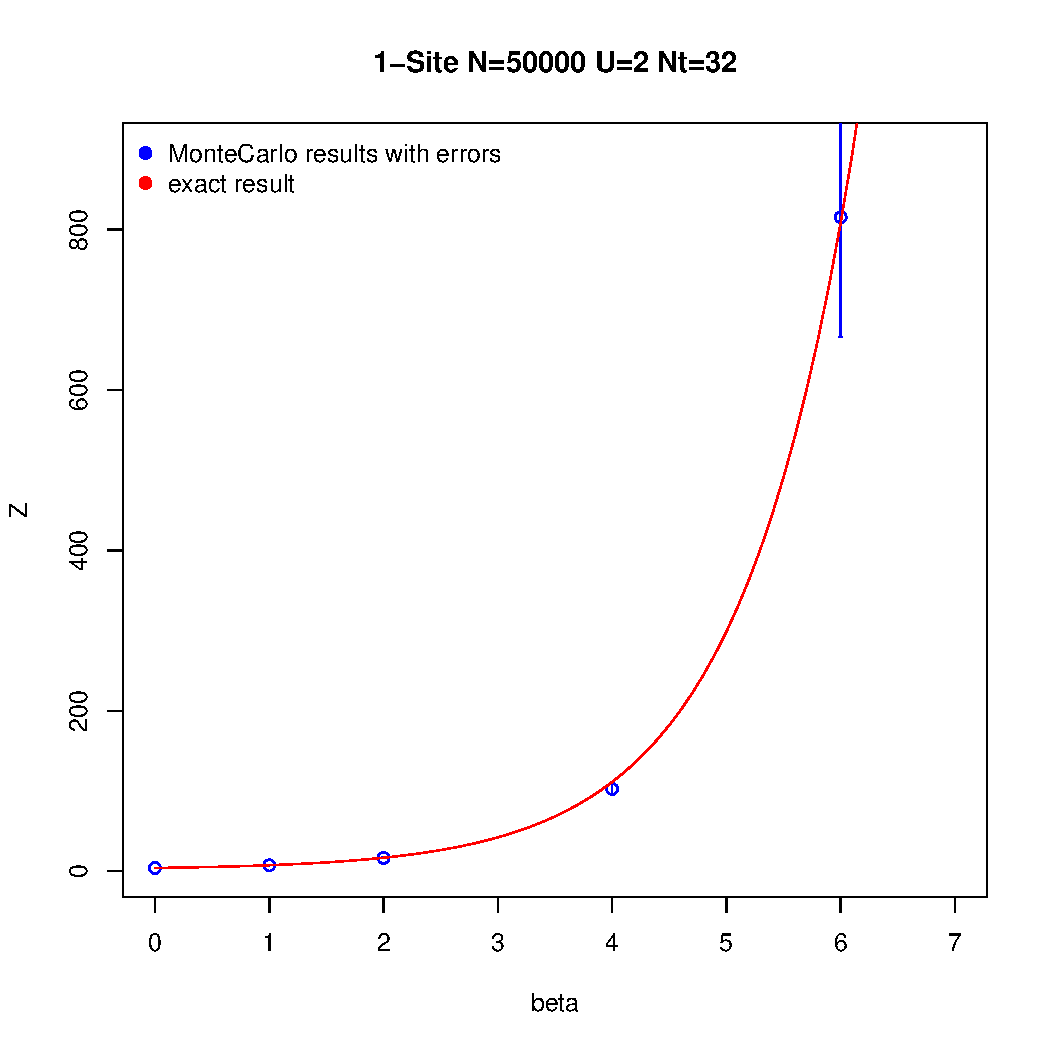
\includegraphics[width=1\linewidth]{figs/plot_Z1b}
			\end{minipage}
		\end{figure}
\end{frame}
\begin{frame}
	\frametitle{Results - Partition function - 2}
	\begin{figure}
		\centering
		\begin{minipage}{.5\textwidth}
			\centering
			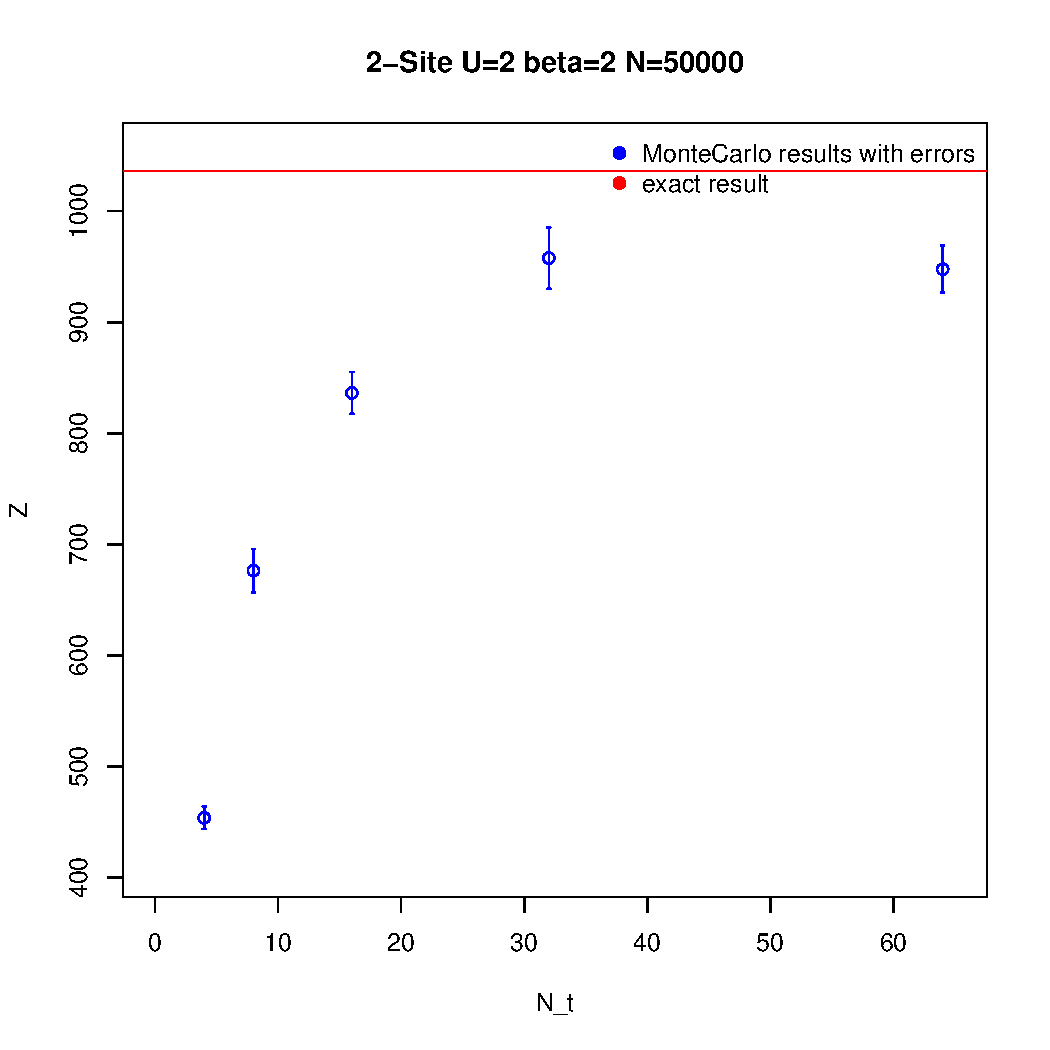
\includegraphics[width=1\linewidth]{figs/plot_Z2Nt}
		\end{minipage}%
		\begin{minipage}{.5\textwidth}
			\centering
			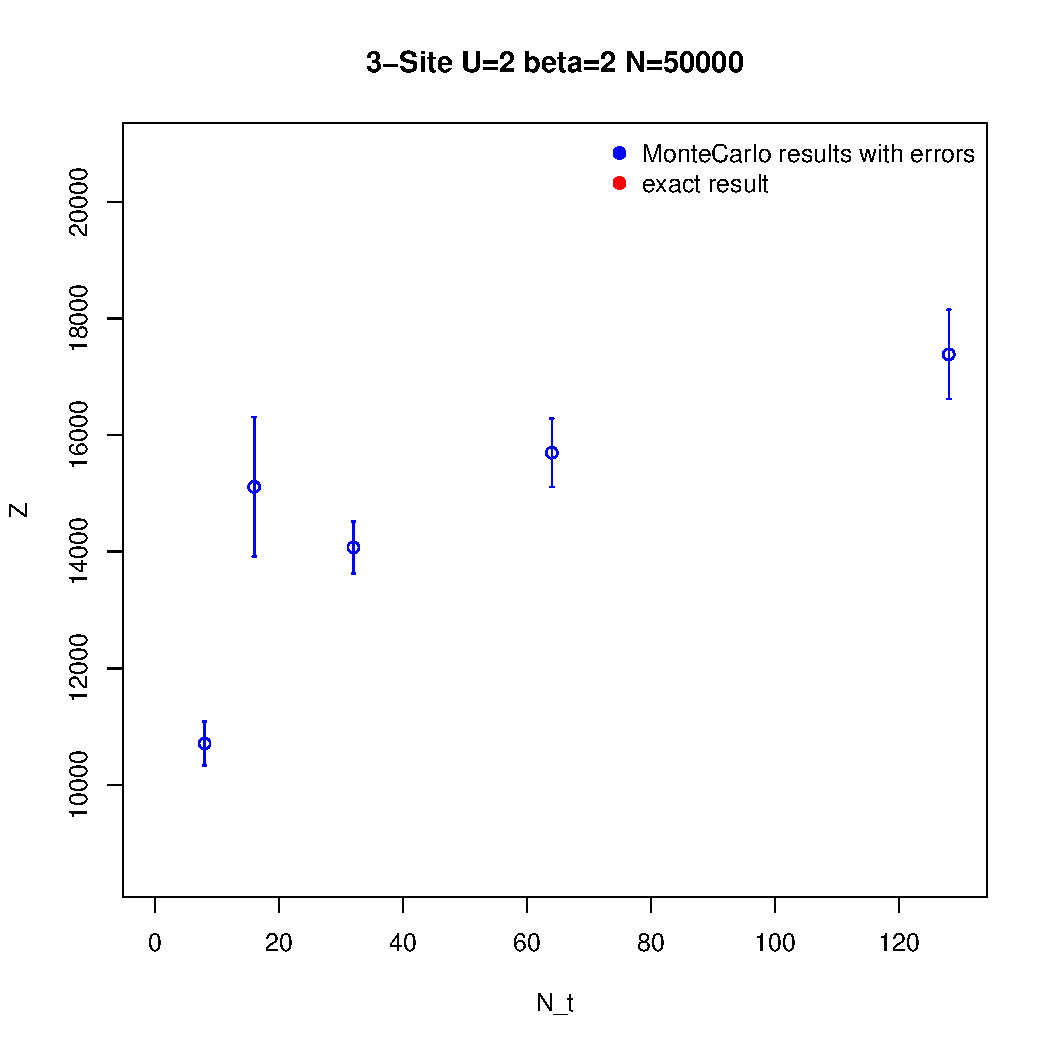
\includegraphics[width=1\linewidth]{figs/plot_Z3Nt}
		\end{minipage}
	\end{figure}
		
\end{frame}

\begin{frame}
	\frametitle{Results - Correlator}
		\begin{figure}
			\centering
			\begin{minipage}{.5\textwidth}
				\centering
				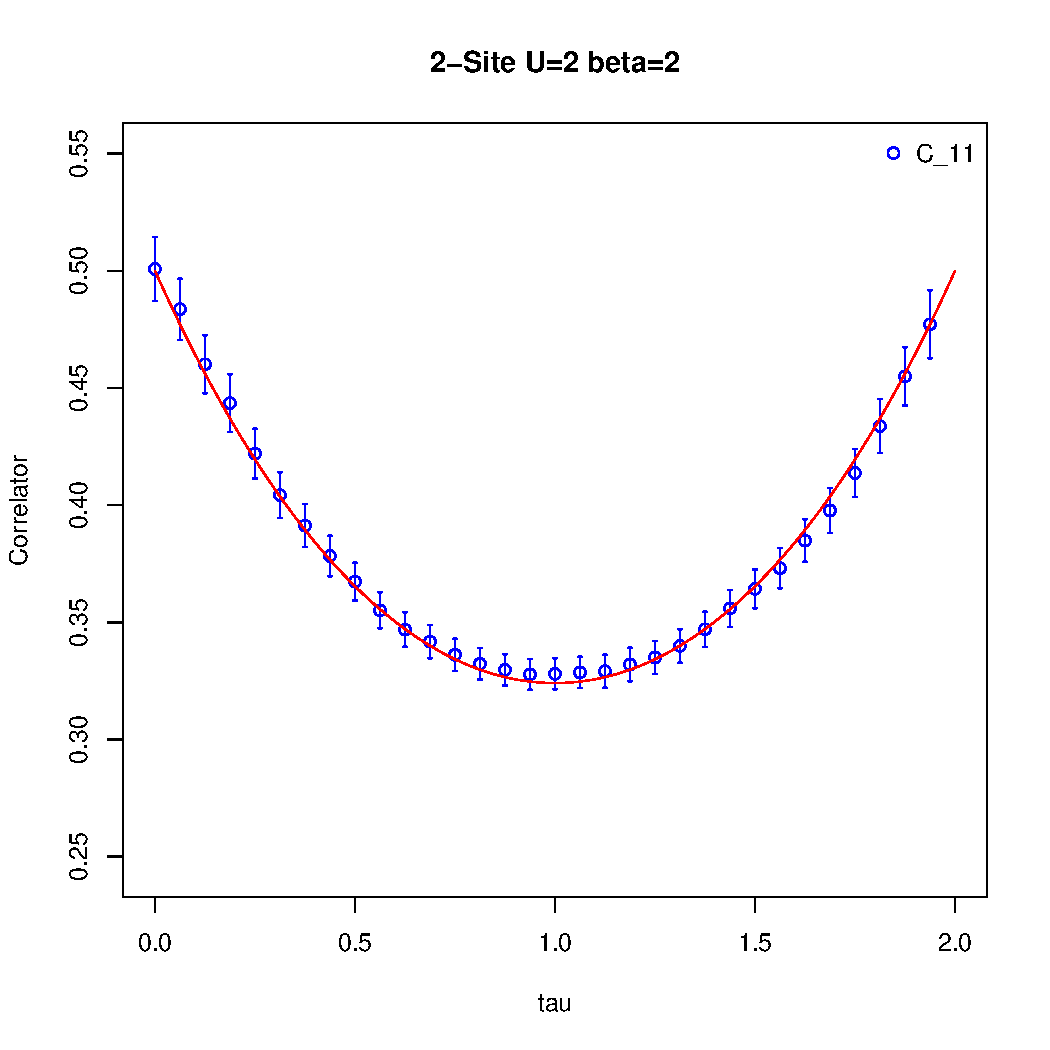
\includegraphics[width=1\linewidth]{figs/plot_C1t}
			\end{minipage}%
			\begin{minipage}{.5\textwidth}
				\centering
				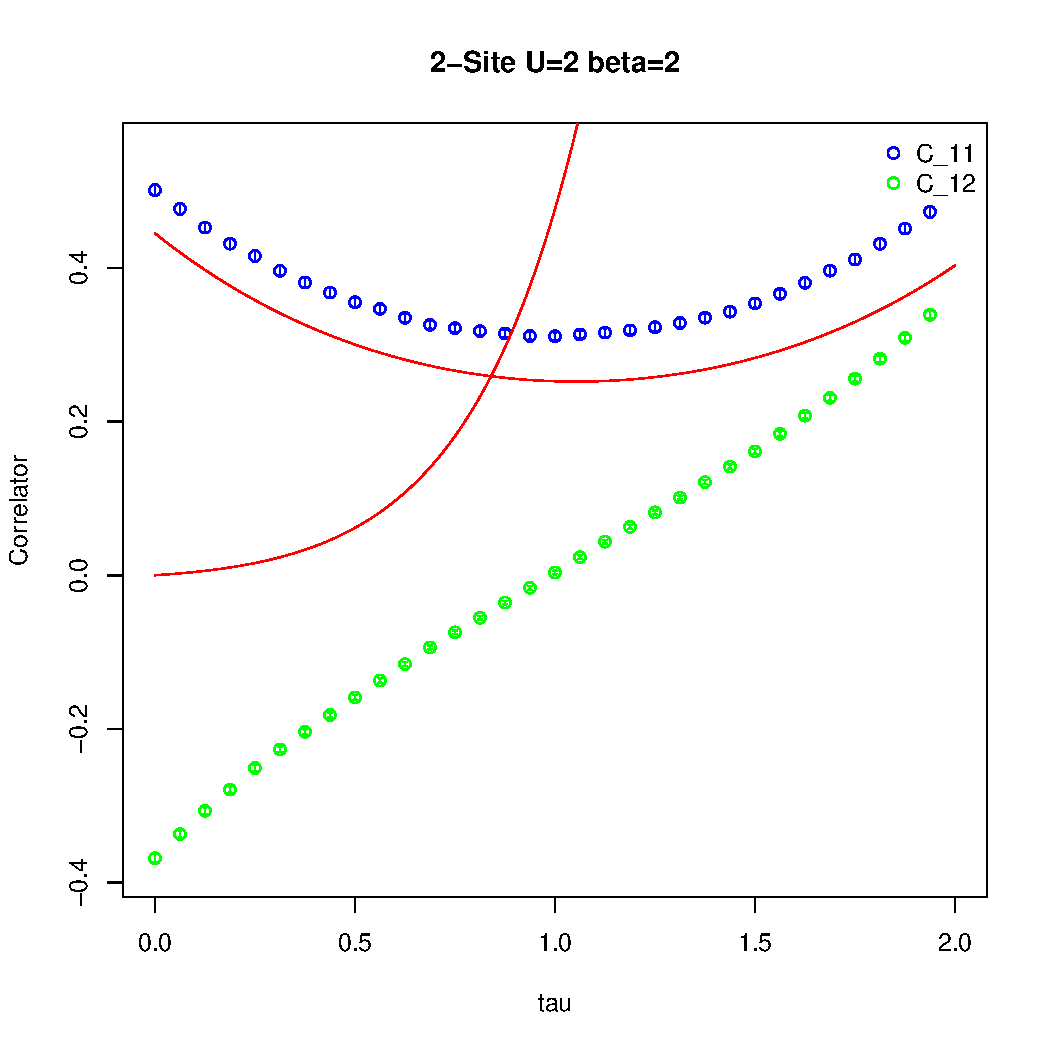
\includegraphics[width=1\linewidth]{figs/plot_C2t}
			\end{minipage}
		\end{figure}
\end{frame}




\section[Conclusion]{Conclusion}
\begin{frame}
\frametitle{Conclusion and Outlook}
\begin{block}{Successes}
\begin{itemize}
\item 1- and 2-site partition function matching 
\item 1- site correlators matching
\item Extension to larger 1D lattices possible 
\end{itemize}
\end{block}

\begin{block}{Outlook}
	\begin{itemize}
		\item Optimize in precision
		\item Optimize in computing time
		\item Higher dimensional model
		\item Grand-canonical ensemble 
	\end{itemize}
\end{block}
\end{frame}

\appendix

\begin{thebibliography}{}
\begin{frame}
\frametitle{References}	
	\bibitem{luu}
	Thomas Luu 2017
	\textit{Fermions and Computers}
	
	\bibitem{lieb}
	E. Lieb, F. Wu 2003
	\textit{The one-dimensional Hubbard model: A Reminiscence}
	
	\bibitem{tasaki} 
	H. Tasaki 1998
	\textit{The Hubbard model - An Introduction and selected rigorous Results}
	
	\bibitem{jafari}
	Seyed A. Jafari 2008
	\textit{Introduction to Hubbard Model and Exact Diagonalization}	
\end{frame}	
\begin{frame}
\frametitle{References - 2}
\bibitem{gabrielsson}
Anders F. Gabrielsson 2011
\textit{Quantum Monte Carlo Simulations of
	the Half-filled Hubbard Model}

\bibitem{Hubbard}
M. Machida et al. \textit{High Performance LOBPCG Method for Solving Multiple Eigenvalues of Hubbard Model: Efficiency of Communication Avoiding Neumann Expansion Preconditioner}
\bibitem{Hubbard2}
\textit{http://atomcool.rice.edu/research/3d-lattice/}
\end{frame}
\end{thebibliography}




\end{document}